\section{Pipeline}

I built the Kerberos pipeline based on excellent explanations at the ZipCPU blog \footcite{ZipCPU.Pipeline}.  Pipeline circuits interface with the skid buffer in a simpler manner than the skid buffer itself interfaces between circuits.

\begin{table}[ht]
    \caption{Handshake State Machine} % title of Table
    \centering % used for centering table
    \begin{tabular}{c c c c c} % centered columns (4 columns)
        \hline\hline
        State & In.Busy & FullBuffer & Out.Strobe & DataOut \\ [0.5ex] % inserts table

        \hline
        Passthrough & 0 & 0 & In.Strobe & Din \\
        Buffer & 1 & 1 & In.Strobe & Din \\
        Flush & 0 & 0 & 1 & Buffer \\ [1ex]
        \hline
    \end{tabular}
    \label{table:pipeline-handshake-circuit-state}
\end{table}

% Pipeline FSM.  Built by hand
\begin{center}
    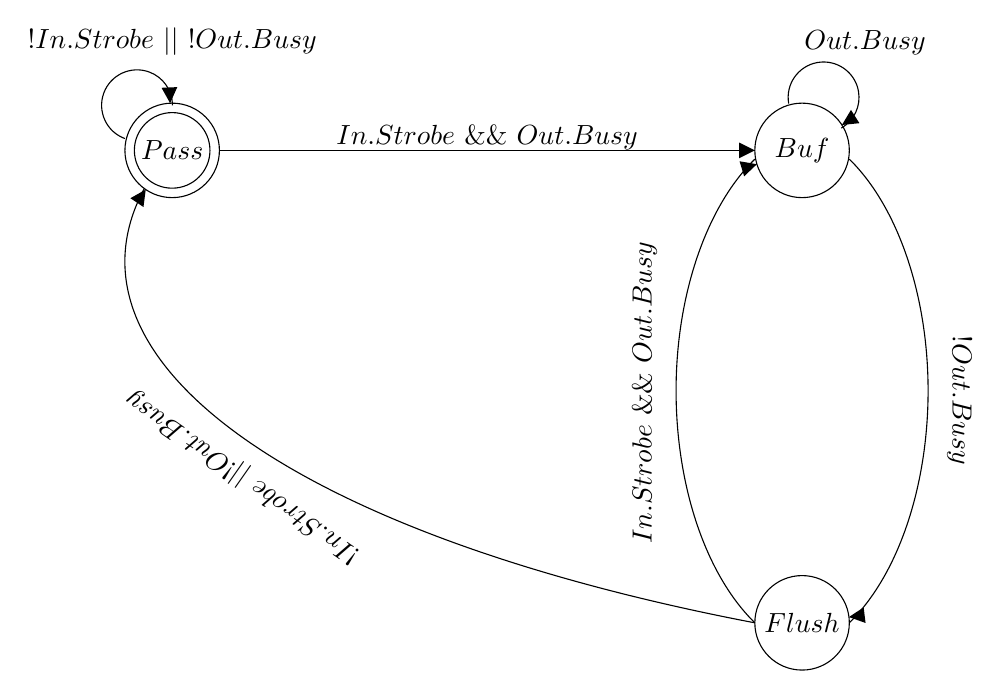
\begin{tikzpicture}[scale=0.2]
    \tikzstyle{every node}+=[inner sep=0pt]

    % Passthrough state
    % XXX:  13.9, -12.4
    \draw [black] (10,-10) circle (3); % Outer circle
    \draw [black] (10,-10) circle (2.4); % Inner accept circle
    \draw (10,-10) node {$Pass$};

    % Buffer state
    \draw [black] (50,-10) circle (3);
    \draw (50,-10) node {$Buf$};

    % Flush state
    % XXX: 39.4, -39.8
    \draw [black] (50,-40) circle (3);
    \draw (50,-40) node {$Flush$};

    % Pass→Pass
    % Arc begin: Outer circle X (10) - radius (3), Outer Circle Y (-10) + (3 - 2.25)
    % Arc start angle: 250, end angle: 0, radius: 2.25
    % End angle found by trial and error
    \draw [black, rotate around={0:(10,-10)}] (7,-9.25) arc (250:0:2.25);
    % Arrowhead: y = outer circe + radius = -10 + 3 (top-center), and +1
    % x = center of circle
    % Up 1, right 0.5; then 0.5 left from there
    \fill [black, rotate around={2.5:(10,-10)}] (10,-7) -- ++(0.5,1) -- ++(-1,0);
    \draw (10,-4) node [above] {$!In.Strobe\mbox{ }||\mbox{ }!Out.Busy$};

    % Pass→Buf
    % Straight line, Y is pass/buff Y, X start is pass + radius (3)
    % length is (()50-3)-(10+3)), the distance between centers plus the offsets,
    % i.e. distance between the connected outer circles.
    \draw [black] (13,-10) -- ++(34,0); %(47,-10);
    \fill [black, rotate around={90:(50,-10)}] (50,-7) -- ++(0.5,1) -- ++(-1,0);
%    \fill [black] (37.7,-12.4) -- (36.9,-11.9) -- (36.9,-12.9);
    \draw (30,-10) node [above] {$In.Strobe\mbox{ }\text{\&\&}\mbox{ }Out.Busy$};

    % Buf→Buf
    % Rotate about its axis…clockwise 90°
    \draw [black, rotate around={-60:(50,-10)}] (47,-9.25) arc (250:0:2.25);
    \fill [black, rotate around={-57.5:(50,-10)}] (50,-7) -- ++(0.5,1) -- ++(-1,0);
    \draw (54,-4) node [above] {$Out.Busy$};

    % Buf→Flush
    % This draws a line of appropriate length to the right and then rotates it 90°.
    % Why? Because drawing diagonal lines is hard, so this is the convention here.
    % It's easy: starting point on the right side, distance to the next circle, rotate.
    %\draw [black, rotate around={-90:(50,-10)}] (53,-10) -- ++(24,0);
    %
    % Or an arc.
    \draw [black, rotate around={0:(50,-40)}] (53,-40) arc (-60:60: 10 and 17);
    \fill [black, rotate around={-83:(50,-40)}] (50,-37) -- ++(0.5,1) -- ++(-1,0);
    \draw (60,-30) node [left, rotate=-90] {$!Out.Busy$};

    % Connector Flush→Buf
    \draw [black, rotate around={0:(50,-40)}] (47,-40) arc (-60:60: -10 and 17);
    \fill [black, rotate around={107:(50,-10)}] (50,-7) -- ++(0.5,1) -- ++(-1,0);
    \draw (40,-35) node [right, rotate=90] {$In.Strobe\mbox{ }\text{\&\&}\mbox{ }Out.Busy$};

    % Connector Flush→Pass
    \draw [black, rotate around={0:(50,-40)}] (47,-40) arc (-60:10: -80 and 26.5);
    \fill [black, rotate around={146:(10,-10)}] (10,-7) -- ++(0.5,1) -- ++(-1,0);
    \draw (15,-30) node [above, rotate=145] {$!In.Strobe\mbox{ }||\mbox{}!Out.Busy$};
    \end{tikzpicture}
\end{center}


Pipelined circuits never simply propagate busy signals:  when the circuit is neither strobing to the next circuit nor processing, it becomes idle.  If the next stage becomes busy, the circuit can still process and wait for a non-busy condition.  These communicate with the pipeline through a simpler state machine with four states:  Idle, Run, Wait, and Finish.

\begin{table}[ht]
    \caption{Execution Circuit State Machine} % title of Table
    \centering % used for centering table
    \begin{tabular}{c c c c c c } % centered columns (4 columns)
        \hline\hline
        State & Processing & DataReady & PipeOut.Busy & PipeIn.Busy \\ [0.5ex] % inserts table

        \hline
        Idle & 0 & 0 & X & 0\\
        Run & 1 & 0 & X & 1 \\
        Wait & 0 & 1 & 1 & 1 \\
        Finished & 0 & 1 & 0 & 0 \\ [1ex]
        \hline
    \end{tabular}
    \label{table:pipeline-exec-circuit-state}
\end{table}

The circuit passes its data on in the Finish state, and is idle on the next iteration; however, the busy signal is \inlinecode{Processing || (DataReady \&\& PipeIn.Busy)}, and so signals \inlinecode{!Busy} on the cycle on which it delivers data.  The \inlinecode{SkidBuffer} itself must accept the data and, besides, is \inlinecode{!Busy} when its buffer is empty and will not magically become busy.

% Built with http://madebyevan.com/fsm/
\begin{center}
    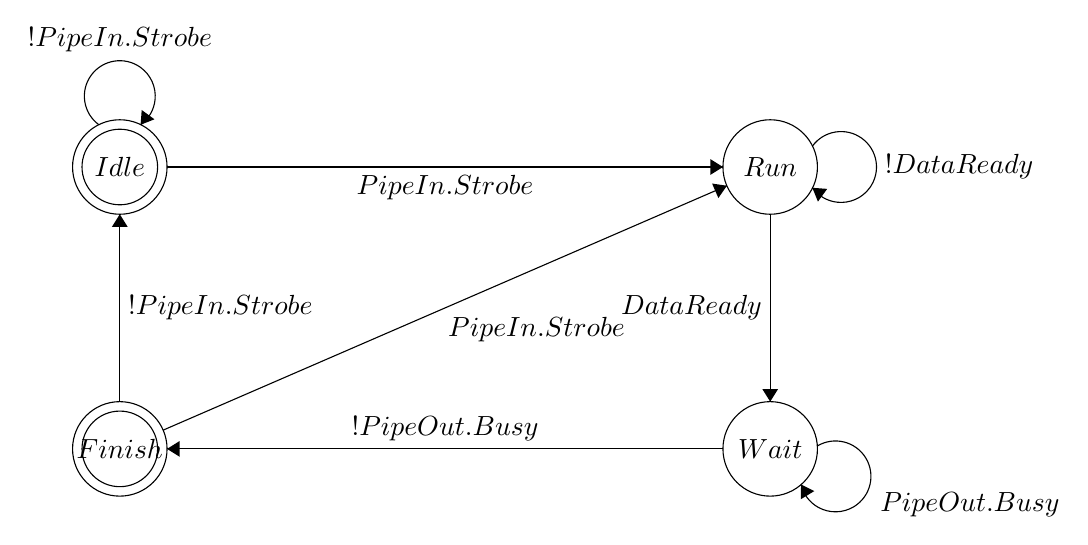
\begin{tikzpicture}[scale=0.2]
    \tikzstyle{every node}+=[inner sep=0pt]
    \draw [black] (11.4,-16.7) circle (3);
    \draw (11.4,-16.7) node {$Idle$};
    \draw [black] (11.4,-16.7) circle (2.4);
    \draw [black] (52.7,-16.7) circle (3);
    \draw (52.7,-16.7) node {$Run$};
    \draw [black] (52.7,-34.6) circle (3);
    \draw (52.7,-34.6) node {$Wait$};
    \draw [black] (11.4,-34.6) circle (3);
    \draw (11.4,-34.6) node {$Finish$};
    \draw [black] (11.4,-34.6) circle (2.4);
    \draw [black] (14.4,-16.7) -- (49.7,-16.7);
    \fill [black] (49.7,-16.7) -- (48.9,-16.2) -- (48.9,-17.2);
    \draw (32.05,-17.2) node [below] {$PipeIn.Strobe$};
    \draw [black] (52.7,-19.7) -- (52.7,-31.6);
    \fill [black] (52.7,-31.6) -- (53.2,-30.8) -- (52.2,-30.8);
    \draw (52.2,-25.65) node [left] {$DataReady$};
    \draw [black] (55.683,-34.421) arc (121.16635:-166.83365:2.25);
    \draw (59.66,-38.16) node [right] {$PipeOut.Busy$};
    \fill [black] (54.66,-36.86) -- (54.64,-37.8) -- (55.5,-37.28);
    \draw [black] (49.7,-34.6) -- (14.4,-34.6);
    \fill [black] (14.4,-34.6) -- (15.2,-35.1) -- (15.2,-34.1);
    \draw (32.05,-34.1) node [above] {$!PipeOut.Busy$};
    \draw [black] (14.15,-33.41) -- (49.95,-17.89);
    \fill [black] (49.95,-17.89) -- (49.01,-17.75) -- (49.41,-18.67);
    \draw (37.86,-26.22) node [below] {$PipeIn.Strobe$};
    \draw [black] (11.4,-31.6) -- (11.4,-19.7);
    \fill [black] (11.4,-19.7) -- (10.9,-20.5) -- (11.9,-20.5);
    \draw (11.9,-25.65) node [right] {$!PipeIn.Strobe$};
    \draw [black] (10.077,-14.02) arc (234:-54:2.25);
    \draw (11.4,-9.45) node [above] {$!PipeIn.Strobe$};
    \fill [black] (12.72,-14.02) -- (13.6,-13.67) -- (12.79,-13.08);
    \draw [black] (55.38,-15.377) arc (144:-144:2.25);
    \draw (59.95,-16.7) node [right] {$!DataReady$};
    \fill [black] (55.38,-18.02) -- (55.73,-18.9) -- (56.32,-18.09);
    \end{tikzpicture}
\end{center}
